\documentclass[master=cws,masteroption=ai]{kulemt}
\setup{title={Describing Images with Natural Language},
  author={Thijs Dieltjens \\ Wout Vekemans},
  promotor={Prof.\,dr.\,ir.\ Marie-Francine Moens},
  assessor={Ir.\,W. Eetveel},
  acyear={2015 -- 2016},
  assistant={Ir.\ S. Zoghbi}}
% De volgende \setup mag verwijderd worden als geen fiche gewenst is.
\setup{filingcard,
  translatedtitle={The best master thesis ever},
  udc=621.3,
  shortabstract={Hier komt een heel bondig abstract van hooguit 500
    woorden. \LaTeX\ commando's mogen hier gebruikt worden. Blanco lijnen
    (of het commando \texttt{\string\pa r}) zijn wel niet toegelaten!
    \endgraf \lipsum[2]}}
% Verwijder de "%" op de volgende lijn als je de kaft wil afdrukken
% \setup{coverpageonly}
% Verwijder de "%" op de volgende lijn als je enkel de eerste pagina's wil
% afdrukken en de rest bv. via Word aanmaken.
%\setup{frontpagesonly}

% Kies de fonts voor de gewone tekst, bv. Latin Modern
\setup{font=lm}

% Hier kun je dan nog andere pakketten laden of eigen definities voorzien

\usepackage{url}
\usepackage{todonotes}
\usepackage{tikz}
% Tenslotte wordt hyperref gebruikt voor pdf bestanden.
% Dit mag verwijderd worden voor de af te drukken versie.
\usepackage[pdfusetitle,colorlinks,plainpages=false]{hyperref}

%%%%%%%
% Om wat tekst te genereren wordt hier het lipsum pakket gebruikt.
% Bij een echte masterproef heb je dit natuurlijk nooit nodig!
\IfFileExists{lipsum.sty}%
 {\usepackage{lipsum}\setlipsumdefault{11-13}}%
 {\newcommand{\lipsum}[1][11-13]{\par Hier komt wat tekst: lipsum ##1.\par}}
%%%%%%%

%\includeonly{hfdst-n}
\begin{document}

\begin{preface}
  Dit is mijn dankwoord om iedereen te danken die mij bezig gehouden heeft.
  Hierbij dank ik mijn promotor, mijn begeleider en de voltallige jury.
  Ook mijn familie heeft mij erg gesteund natuurlijk.
\end{preface}

\tableofcontents*

\begin{abstract}
  In dit \texttt{abstract} environment wordt een al dan niet uitgebreide
  samenvatting van het werk gegeven. De bedoeling is wel dat dit tot
  1~bladzijde beperkt blijft.

  \lipsum[1]
\end{abstract}                                                                                                                                                                                                                                                                                                                                                                                                                                                                                                                                                                                                                                                                                                                 

% Een lijst van figuren en tabellen is optioneel
%\listoffigures
%\listoftables
% Bij een beperkt aantal figuren en tabellen gebruik je liever het volgende:
\listoffiguresandtables
% De lijst van symbolen is eveneens optioneel.
% Deze lijst moet wel manueel aangemaakt worden, bv. als volgt:
\chapter{Lijst van afkortingen en symbolen}
\section*{Afkortingen}
\begin{flushleft}
  \renewcommand{\arraystretch}{1.1}
  \begin{tabularx}{\textwidth}{@{}p{12mm}X@{}}
    LDA  & Latent Dirichlet Allocation \\
    RNN & Recurrent Neuraal Netwerk \\
    CNN & Convolutioneel Neuraal Netwerk \\
    LSTM & Long Short Term Memory \\
    CCA & Canonical Correlation Analysis \\
    RFF & Random Fourier Feature
    
    
  \end{tabularx}
\end{flushleft}


\section*{Symbolen}
\begin{flushleft}
  \renewcommand{\arraystretch}{1.1}
  \begin{tabularx}{\textwidth}{@{}p{12mm}X@{}}
    $\theta$   & Kansverdeling van onderwerpen per document (LDA) \\
    $\phi$   & Kansverdeling van woorden per onderwerp (LDA)  \\
  \end{tabularx}
\end{flushleft}

% Nu begint de eigenlijke tekst
\mainmatter

\chapter{Inleiding}
\label{inleiding}
In dit hoofdstuk wordt het werk ingeleid. Het doel wordt gedefinieerd en er
wordt uitgelegd wat de te volgen weg is (beter bekend als de rode draad).

Als je niet goed weet wat een masterproef is, kan je altijd
Wikipedia\cite{wiki} eens nakijken.

\section{Lorem ipsum 4--5}
\lipsum[4-5]

\section{Lorem ipsum 6--7}
\lipsum[6-7]

%%% Local Variables: 
%%% mode: latex
%%% TeX-master: "masterproef"
%%% End: 

\chapter{Gerelateerd werk}
\label{hoofdstuk:related}
Het automatisch genereren van beschrijvingen voor ongeziene afbeeldingen is een complex proces. Het combineert namelijk zowel computervisie (CV) als natuurlijke taalverwerking (NLP). Vele modellen zijn al voorgesteld die telkens elementen uit beide onderzoeksvelden combineren. 

Dit hoofdstuk begint met een vergelijking van verschillende mogelijkheden om afbeeldingen en zinnen voor te stellen. De meest relevante onderzoeken uit CV en NLP komen aan bod. Daarna volgt een samenvatting van de verschillende mogelijkheden om deze technologie\"en te integreren in \'e\'en model. 

Doorheen de jaren is deze integratie op verschillende manieren aangepakt. Het probleem van automatische afbeeldingsbeschrijving werd eerst niet beschouwd als generatieprobleem maar als opvraag- of \emph{retrievalprobleem}. Hierbij zoekt een model naar de beste zin in een bestaande verzameling van zinnen op basis van de ingevoerde foto \cite{Hodosh2013}. Nieuwere papers behandelen het probleem als een vertaalprobleem naar analogie met automatisch vertalen. Hierbij gebruikt men een codeer-decodeersysteem waarbij de afbeelding als brontaal wordt beschouwd en het Engels als doeltaal. Dit hoofdstuk biedt een overzicht van deze recentste technieken.

\section{Representatie van afbeeldingen}
Alle recente modellen gebruiken technieken uit computervisie om nuttige kenmerken af te leiden uit afbeeldingen. Kenmerken bevatten onder andere gedetecteerde acties, sc\`enes en objecten met hun attributen en relaties\cite{Bernardi}. Deze kenmerken vormen de basis voor een representatie van de afbeelding die als input dient voor het generatie- of opvraagmodel.

Eerst volgt een bespreking van technieken uit het verleden. Daarna beschrijft deze sectie Convolutionele Neurale Netwerken (CNN), die in de meer recente literatuur veelvuldig voorkomen.


\subsection{Oorspronkelijke CV modellen}
De literatuur gebruikt meerdere technieken uit computervisie om nuttige features of kenmerken af te leiden uit afbeeldingen. Kenmerken die in de vroegste papers over dit onderwerp voorkomen zijn bijvoorbeeld het type van de algemene sc\`ene, gedetecteerde objecten en attributen van deze objecten\cite{Farhadi2010,Patterson2014,Yang2011}.

Bij sc\`eneclassificatie leert een model voor ongeziene afbeeldingen een bepaalde algemene sc\`ene (bijvoorbeeld restaurant, slaapkamer, keuken) af te leiden. Ook modellen die verschillende objecten detecteren hebben hun nut. Van zulke gevonden objecten kunnen classifiers ook nog nuttige attributen zoals kleur bepalen. Om zulke afleidingen te maken, gebruiken de papers bestaande classifiers en detectoren zoals bij Felzenswalb et al.\cite{Felzenszwalb2008}, Im2Text\cite{Ordonez2011} en GIST\cite{Oliva2006}. Ee\'n of meerdere van deze features kan dan rechtstreeks de representatie vormen van een afbeelding. Daarnaast vormen deze features in een aantal werken\cite{Farhadi2010,Li2011,Mitchell2012,Yang2011} enkel de input voor abstracte afbeeldingsrepresentaties in de vorm van tupels. Deze tupels bevatten dan objecten, acties tussen objecten, sc\`enetypes en/of ruimtelijke relaties.

Een andere manier om afbeeldingen voor te stellen is het gebruik van Visual Dependency Representations (VDR) zoals voorgesteld door Elliott et al.\cite{Elliott2013}. Dit model werkt analoog aan een taalgebaseerde afhankelijkheidsgrammatica. Dit type grammatica stelt de syntactische structuur van een zin voor met woorden met daartussen binaire semantische of syntactische relaties\cite{Jurafsky:2009:SLP:1214993}. Figuur \ref{fig:dep_grammar} toont een voorbeeld van een zin ontleed met een afhankelijkheidsgrammatica. De gelabelde pijlen stellen de verschillende relaties tussen de woorden voor.

\begin{figure}[tb]
      \centering
      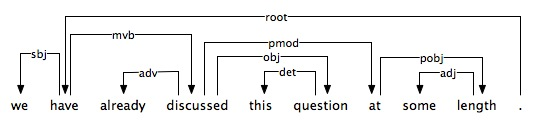
\includegraphics[width=\linewidth]{Images/dependencygrammar.jpg}
      \caption{Zin ontleed met afhankelijkheidsgrammatica\cite{GasserNotes}}
      \label{fig:dep_grammar}
  \end{figure}  

VDR's gebruiken een afhankelijkheidsgraaf om de ruimtelijke relaties tussen regio's in een foto voor te stellen. Elke relatie tussen twee objecten krijgt dan een ruimtelijke positie als label. Mogelijke relaties zijn bijvoorbeeld \texttt{op}, \texttt{boven}, \texttt{onder}, \texttt{naast}, ... Het leren van VDR's kan op basis van geannoteerde trainingsdata, automatisch met objectherkenning\cite{Elliott2015} of met nog andere informatie die in de abstracte sc\`ene zit\cite{Gilberto2015}.  

\todo[inline]{Framenet vermelden?}

\subsection{CV met neurale netwerken}
Naast deze meer traditionele manieren om informatie uit afbeeldingen af te leiden, bieden neurale netwerken een alternatieve oplossing. Voor een theoretische uitwerking van de gebruikte neurale netwerken, zie hoofdstuk \ref{hst-theorie}.

Voor de meeste taken binnen computervisie blijkt dat convolutionele neurale netwerken (CNN) beter presteren dan bovenstaande methodes.\todo{hier sta iets bij geschreven, ik denk dat het ``hoe?'' is} Deze CNN's zijn deep learning neurale netwerken met soms meer dan 15 verborgen lagen. Ze hebben minder verbindingen en parameters dan overeenkomstige feedforward neurale netwerken terwijl ze niet veel slechter presteren\cite{Krizhevsky2012a}. 
Voor verschillende CV-taken werken de huidige state-of-the-art oplossingen op basis van CNN's. Dit is onder andere het geval voor gezichtsherkenning\cite{Zhou2015}, tekenherkenning\cite{Ciresan2012} en objectherkenning\cite{Szegedy2014}.

De gebruikte CNN's binnen het automatisch beschrijven van afbeeldingen zijn getraind op ImageNet\cite{Russakovsky2014}. ImageNet is een dataset bestaande uit miljoenen afbeeldingen die gelabeld zijn binnen enkele duizenden categorie\"en. Het neuraal netwerk leert afbeeldingen correct te classificeren. Vaak gebruikte CNN modellen zijn AlexNet\cite{Krizhevsky2012a} en het recentere VGGNet\cite{Arge2015}.

Elke afbeelding dient als input voor het netwerk om zo tot een representatieve vector te komen. De meeste papers die afbeeldingen beschrijven gebruiken de gewichten van de laag voor de uiteindelijke classificatie als representatie van een afbeelding\cite{Chen2014,Karpathy2015,Mao2014a,Google}. Aandachtsgebaseerde oplossingen\cite{Jin2015,Xu2015} gebruiken ook de output van lagere convolutionele lagen als extra informatie.

Regionale CNN's vormen een variatie op CNN die een afbeelding opdeelt in verschillende interessante regio's. Hiermee is het mogelijk om voor elke regio een representatie te maken\cite{Karpathy2015,Mitchell2015}. 

\section{Representatie van zinnen}
Het is niet eenvoudig om rechtstreeks met zinnen als een geheel te werken. Daarom zijn er verschillende alternatieven onderzocht om een zin voor te stellen.
De meeste modellen vertrekken van een vectorrepresentatie voor individuele woorden. In de literatuur zijn er verschillende manieren beschreven om woordrepresentaties samen te voegen tot een representatie van een zin.

\subsection{Voorstellen van woorden}
 Het voorstellen van woorden met een vector vergemakkelijkt de verdere verwerking en kan bovendien ook semantische informatie bevatten.

 Een eerste mogelijke voorstelling is een one-hot codering waarin een vector met als grootte het aantal woorden in het vocabularium elk woord voorstelt. Deze vector is volledig nul behalve op \'e\'en rij die overeenkomt met het woord. Het is mogelijk om deze representatie verder uit breiden door vermenigvuldiging met een gewichtsmatrix. Deze matrix transformeert de one-hotvectoren naar een andere vector. Training kan zorgen voor aanpassingen aan deze gewichtsmatrix om zo ook de semantische informatie van de woorden te leren. Deze gewichtsmatrix kan willekeurig worden ge\"initialiseerd of eerst trainen op bestaande corpora\cite{Lebret2013,Mao2014a,Google}. Daarna kunnen de gekende woorden en zinnen uit de dataset de gewichten nog verfijnen.  

 Een andere mogelijkheid is om bestaande word embeddings te gebruiken zoals \texttt{word2vec}. Dat algoritme projecteert elk woord op een vooraf geleerde vector en heeft bovendien enkele mooie eigenschappen. Zo projecteert het semantisch gelijkaardige woorden op nabijgelegen posities in de vectorruimte\cite{Mikolov2013}. Deze voorgedefin\"ieerde vectoren hebben als nadeel dat niet voor elk woord uit de beschrijvingen een vector representatie beschikbaar is. Het is wel mogelijk om zelf de vectorrepresentaties te leren op basis van de gebruikte dataset zoals beschreven in de paper.

 De meeste werken in de literatuur rapporteren dat one-hotcodering in combinatie met een te leren gewichtsmatrix gelijkaardige en snellere resultaten oplevert. Daarnaast hebben sommige semantisch gelijkaardige woorden zoals kleuren gelijkaardige vectoren bij gebruik van het \texttt{word2vec} algoritme, terwijl kleuren in een afbeelding toch uitgesproken verschillend zijn. Hierdoor zal een systeem dat \texttt{word2vec} woordvectoren gebruikt, waarschijnlijk slecht presteren in het herkennen van kleuren\cite{Karpathy2015}.
 
\subsection{Voorstellen van zinnen}
 Verschillende mogelijkheden bestaan om de zinnen voor te stellen wanneer de woordvectoren gekend zijn. Een eerste mogelijkheid gebruikt een afhankelijkheidsparser en stelt de zinnen voor als een volledige afhankelijkheidsboom\cite{Socher2014}. Karpathy\cite{Karpathy2014} gebruikt ook een afhankelijkheidsparser, maar haalt hier een verzameling van triplets uit. Dergelijke triplets bestaan uit twee woorden uit de zin en hun onderlinge relatie. Figuur \ref{fig:deprelations} toont een voorbeeldzin met de bijhorende triplets. Het eerste element van de triplet is het type van de relatie.

 \begin{figure}[tb]
     \centering
     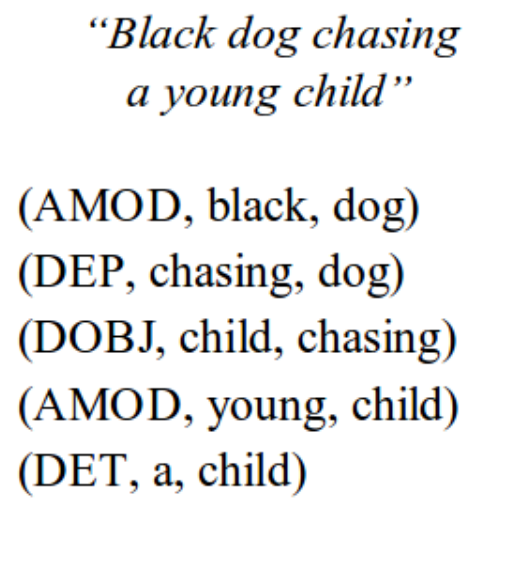
\includegraphics[width=0.35\textwidth]{Images/dep_relations}
     \caption{Zin met ontlede afhankelijkheidstriplets\cite{Karpathy2014}}
     \label{fig:deprelations}
 \end{figure}

 Een volgende optie telt de woordvectoren van een zin op\cite{Lebret2013}  Hierdoor gaat informatie uit de woordvolgorde wel verloren. Le en Mikolov\cite{Le2014a} bieden een oplossing voor het verloren gaan van woordvolgorde. Zij trainen een model om representaties te maken van stukken tekst met variabele lengte. Hun algoritme kan zowel zinnen als paragrafen en volledige teksten voorstellen.

 Een vaak gebruikt taalmodel in de meer recente NLP-literatuur is een Recurrent Neuraal Netwerk (RNN)\cite{Mikolov2010}. Dit is een neuraal netwerk dat goed overweg kan met sequenti\"ele data zoals taal. Kiros et al.\cite{Kiros2013} combineren de verborgen lagen van een RNN met extra informatie (zoals POS-tags) om tot een representatie van de zin te komen. De meer recente modellen stellen een zin voor als de sequentie van de woordvectoren in die zin. Zo kan het RNN de taal leren door elke zin woord per woord in het netwerk in te voeren.
 
\section{Van afbeeldingsrepresentaties naar beschrijvingen}
Er zijn verschillende methodes om vanuit de representaties van de afbeelding en bijbehorende referentiezinnen een model te trainen dat in staat is om ongeziene afbeeldingen om te zetten in correcte beschrijvingen. 
De meeste modellen trainen met als doel het verschil tussen de gegenereerde omschrijving en de correcte omschrijving uit de trainingsverzameling te minimaliseren.

\subsection{Dichtstbijzijnde afbeelding}
De eenvoudigste aanpak zoekt naar de meest gelijkaardige afbeelding in de trainingsverzameling en geeft \'e\'en van haar beschrijvingen terug als resultaat(Nearest Neighbour)\cite{Devlin2015a}. Een gelijkaardigheidsmetriek zoals de cosinusgelijkenis tussen de afbeeldingsrepresentaties evalueert de gelijkaardigheid van twee representaties.

Een uitbreiding op deze aanpak zoekt naar de verzameling van de meest gelijkaardige afbeeldingen in de trainingsverzameling. Vervolgens cre\"eert een model een rangorde op basis van extra visuele of tekstuele informatie. De referentiezin van de hoogst scorende afbeelding is dan het resultaat\cite{Devlin2015a,Hodosh2013,Oliva2006,Ordonez2011}. 
Deze modellen hebben als nadeel dat ze nooit resulteren in een zin die niet in de trainingsverzameling zit.

Een variatie hierop gebruikt een afbeeldingsvoorstelling met gedetecteerde objecten. Dit systeem zoekt naar de beschrijving van visueel gelijkaardige objecten in de vorm van zinsfragmenten (frases)\cite{Gupta2012,Kuznetsova2012}. Met de verzamelde fragmenten zoekt het systeem dan de meest waarschijnlijke nieuwe zin op basis van het type van de fragmenten. Deze types bestaan uit naamwoordsgroep (NP), werkwoordsgroep (VP) en voorzetselgroep (PP). De samenstelling van een nieuwe zin gebeurt dus op basis van zinsdelen die objecten gelijkaardig aan die op de foto beschrijven. De auteurs defin\"ieren meerdere beperkingen op de gegeneerde zinnen om het aantal mogelijkheden te verkleinen.

Een andere variatie op Nearest Neighbour geeft de zinnen, samen met de dichtstbijzijnde afbeelding, als input aan een tweede model. Dit model vormt deze informatie dan om tot een nieuwe zin. Zo beschouwen Mason et al.\cite{Mason2014} het genereren van beschrijvingen als een samenvattingsprobleem en gebruiken ze de beschrijvingen van gelijkaardige afbeeldingen als extra input. Analoog verkrijgen Jia et al.\cite{Fernando2015} verbeteringen op bestaande modellen door het toevoegen van extra semantische informatie zoals beschrijvingen van gelijkaardige afbeeldingen op basis van Canonical Correlation Analysis (CCA).
 
\subsection{Multimodale modellen}
Enkele werken proberen een gemeenschappelijke ruimte tussen zinnen en afbeeldingen te leren zodat het mogelijk is om de representatie van zinnen zowel als afbeeldingen op dezelfde ruimte te projecteren. Dit laat toe om afbeeldingen en zinnen rechtstreeks te vergelijken met een afstandsmaat zoals bijvoorbeeld de cosinusgelijkenis. Dit is zeer nuttig voor onder andere het opvragen van afbeeldingen met een ongeziene query en zinnen met een ongeziene afbeelding. Het leren van multimodale modellen kan onder andere met Canonical Correlation Analysis (CCA)\cite{Hodosh2013} en neurale netwerken\cite{Mao2014,Karpathy2014,Kiros2013}. 

\subsection{Sjabloongebaseerd}
Een volgende aanpak baseert zich op sjablonen om zinnen te genereren. Op basis van de gebruikte afbeeldingsvoorstelling vult een algoritme een voorgedefinieerd sjabloon in\cite{Yang2011}. Hiervoor is het dikwijls nodig om bijkomende complexe modellen te trainen\cite{Elliott2013}. Het nadeel van deze methode is dat de gegenereerde zinnen wel syntactisch correct zijn, maar dikwijls onnatuurlijk aanvoelen voor mensen. Om deze methode te verbeteren kunnen gegenereerde of vooraf gekende zinsfragmenten helpen bij het hercombineren van fragmenten\cite{Mitchell2012,Kuznetsova2012}. Daarnaast kan een algoritme een aantal gegenereerde zinnen sorteren op basis van verschillende factoren en zo de beste zin eruit halen. \todo{voorbeeld van deze factoren}

\subsection{Neurale netwerken}
De meest recente en best scorende modellen gebruiken neurale netwerken als taalmodel voor het genereren van beschrijvingen. Deze taalmodellen zijn in staat om compleet nieuwe, vlotte en natuurlijk aanvoelende zinnen te produceren. Vooral Recurrente Neurale Netwerken (RNN)\cite{Mikolov2010} winnen in de literatuur aan populariteit als taalmodel. RNN's zijn in staat om sequenti\"ele data te genereren op basis van een zekere input. LSTM's (Long Short Term Memory)\cite{SeppHochreiter1997} vormen een uitbreiding op de RNN's en onthouden informatie op lange termijn met behulp van een geheugencel.

Beide modellen verwachten een sequentie van woordrepresentaties als input, maar kunnen ook uitgebreid worden met extra informatie als invoer. Zo gebruiken meerdere werken de afbeelding als eerste invoer. Een andere toevoeging cre\"eert een multimodale ruimte tussen afbeeldingen en zinnen\cite{Kiros2014,Socher2014}. Xu et al.\cite{Xu2015} voegen een ``aandachtsvector'' toe die aangeeft waar in de afbeelding het systeem moet focussen. Het is ook mogelijk om een combinatie van verschillende technieken te gebruiken, zoals het leren van een ``sc\`enevector'' in combinatie met een aandachtsgebaseerd systeem\cite{Jin2015}. Jia et al. experimenteren met verschillende mogelijkheden om extra informatie toe te voegen, zoals CCA-projecties van afbeeldingen, of de afbeelding zelf\cite{Fernando2015}.

Een eerste verzameling van modellen met neurale netwerken volgt het codeer-decodeerprincipe uit de automatische vertaling\cite{Kiros2014}. De codeercomponent transformeert een afbeelding naar een nieuwe (multimodale) representatie. De decodeercomponent vertaalt vervolgens deze multimodale representatie naar een zin in natuurlijke taal. Door het multimodale karakter van deze modellen is het opvragen van afbeeldingen en zinnen ook mogelijk. Dit opvragen gebeurt door middel van projectie van een nieuwe afbeelding of zin in de multimodale ruimte. Een vergelijking van deze projectie met de zinnen of afbeeldingen uit de trainingsverzameling leidt tot een rangschikking van de trainingsvoorbeelden. Er bestaan zowel codeer-decodeer modellen met LSTM's\cite{Kiros2014} als met RNN's\cite{Karpathy2014,Mao2014a}.

Een tweede categorie gebruikt zowel de afbeeldingsrepresentatie als de sequentie van 
woordrepresentaties als input bij het trainen van het netwerk. Op basis van een trainingsafbeelding probeert het netwerk het eerste woord uit de zin te voorspellen. Deze voorspelling dient dan, al dan niet samen met de afbeelding, als input voor de voorspelling van het volgende woord. Terugpropagatie van de fout op de gegenereerde woorden doorheen het netwerk zorgt voor de juiste wijzigingen aan de gewichten. Op deze manier leert het netwerk om op basis van een ongeziene afbeelding de juiste sequentie van woorden te genereren. Ook hier bestaan er modellen met LSTM's\cite{Donahue2015,Google} en RNN's\cite{Karpathy2015}. \todo{meer papers toevoegen}

Het trainen van deze netwerken gebeurt doorgaans met terugpropagatie doorheen het netwerk. Het is mogelijk om de fouten ook verder door te propageren naar de gewichtsvectoren van de woordrepresentaties of naar de gewichten van een CNN. Die methode optimaliseert op die manier alle gewichten op de dataset, maar kan computationeel kostelijk zijn.

Alle neurale netwerken gebruikt in deze thesis hebben een ``softmax'' als laatste laag. Deze laag zorgt ervoor dat het netwerk een kansverdeling genereert voor het volgende woord. Het meest waarschijnlijke woord heeft dan de hoogste kans.
Het selecteren van het woord voor de generatie kan gebeuren door het samplen van deze verdeling, of door het gebruik van een zoekalgoritme zoals beam search, om zo de meest waarschijnlijke beschrijving te benaderen. Een specifiek stopwoord kenmerkt zowel het begin als het einde van de zin.

\subsection{Statistische taalmodellen}
Naast de neurale netwerken behoren ook de statistische taalmodellen tot de beter scorende modellen. Deze modellen proberen op basis van entropie een taal zo goed mogelijk te beschrijven. Entropie is een maat voor informatie en heeft verschillende doeleinden binnen het domein van NLP. 

Concreet stelt de entropie $H$ de hoeveelheid informatie voor die in een willekeurige variabele $X$ zit. $X$ is typisch de voorspelde variabele. Bij het afbeeldingsbeschrijvingsprobleem zijn dit typisch woorden of zinnen. Het domein van deze variabele is $\chi$. De entropie van $X$ is te berekenen met formule \eqref{entropy}, waarbij $p(x)$ de kans voorstelt dat $X$ waarde $x$ heeft\cite{Jurafsky:2009:SLP:1214993}. 

\begin{equation}
     H(X) = -\sum_{x \in \chi}p(x)\log_2p(x)
     \label{entropy}
 \end{equation} 

Entropie-gebaseerde modellen modelleren de kennis die zeker is en ze beschouwen onzekerheden als uniform. Als een woord vijf mogelijke vertalingen heeft, waar het systeem verder niets over weet, heeft elke vertaling een kans van $\frac{1}{5}$. Als het systeem uit observatie weet dat in 50 \% van de gevallen een van de eerste 2 vertalingen is, hebben deze twee vertalingen een waarschijnlijkheid van $\frac{1}{4}$. De andere drie vertalingen, waarover het systeem onzeker is, hebben een waarschijnlijkheid van $\frac{1}{6}$, wat neerkomt op een uniforme kansverdeling binnen de beperkingen die uit de observaties voortkomen. In andere modellen kunnen deze beperkingen voortkomen uit sjablonen, het al dan niet observeren van bepaalde woordsequenties, \ldots \cite{Berger1996}

Zo leren Mitchell et al.\cite{Mitchell2015} om een lijst met waarschijnlijke woorden uit de afbeeldingsrepresentatie te extraheren en combineren ze deze met een uitgebreid taalmodel. Dit taalmodel leert de verschillende kansen op basis van de beschrijvingen in de trainingsdata. Tijdens het leerproces probeert het algoritme de entropie te maximaliseren. In een volgende stap van hun systeem zoeken ze de zinnen die het meest waarschijnlijk zijn, gegeven de woorden die herkend zijn in de afbeelding. Vervolgens sorteren ze de gegeneerde zinnen op basis van een aantal additionele kenmerken. Dit model is net als de modellen met neurale netwerken in staat om nieuwe en vlotte zinnen te vormen. De prestatie is gelijkaardig aan die van de neurale netwerken.

Lebret\cite{Lebret2015} toont bovendien aan dat een nog eenvoudiger taalmodel toch relatief goede resultaten kan bekomen. Dit model extraheert alle zinsfragmenten (frases) uit de trainingsdata en leert daarmee een eenvoudig 3-gram taalmodel. Voor ongeziene afbeeldingen bepaalt het model de best overeenkomende zinsfragmenten en probeert hiermee zinnen te maken. In tegenstelling tot alle voorgaande modellen gebeurt training van deze multimodale transformatie met negatieve sampling. Hierbij leert het model een juiste referentiezin te onderscheiden in een lijst die ook willekeurig gekozen zinnen bevat. Ook hier gebeurt er aan het einde nog een hersortering van de gegenereerde zinnen op basis van de overeenstemming met de afbeelding.

\subsection{Aandachtsgebaseerde modellen}
State-of-the-art modellen uit het automatisch vertalen gebruiken mechanismes die aandachtsgebaseerd zijn. Concreet betekent dit dat het decodeeralgoritme zelf beslist welke stukken uit de zin meer aandacht vereisen.
In de setting van het beschrijven van afbeeldingen komt dit neer op een mechanisme dat aangeeft welke regio's in de afbeelding belangrijk zijn. In de decoder zorgt dit aandachtsmechanisme voor een extra contextvector als input voor een neuraal netwerk. 

Deze aandachtsvector kan zowel ``hard'' als ``zacht'' zijn. ``Harde'' aandacht is een stochastisch principe dat de aandachtslocatie beschouwt als een latente variabele. Tijdens elke stap samplet\todo{Nederlands woord?} het algoritme \'e\'en locatie om de aandacht op te vestigen tijdens het genereren van het volgende woord. ``Zachte'' aandachtsmethodes werken deterministisch, waardoor er geen nood is om elke stap een sample-operatie uit te voeren. Een differentieerbare functie bepaalt de aandachtslocatie tijdens elke stap van het trainingsproces. Door de differentieerbaarheid is het netwerk dat de aandachtsvector berekent eenvoudig te trainen met behulp van terugpropagatie.

Aandachtsmodellen geven bovendien een mooie visuele voorstelling van waar het model bepaalde woorden ``ziet'' (figuur \ref{fig:attention-example}). Binnen het automatisch beschrijven van afbeeldingen bereiken deze aandachtsgebaseerde modellen voorlopig de beste resultaten\cite{Jin2015,Xu2015}.

\begin{figure}[tb]
	\centering
	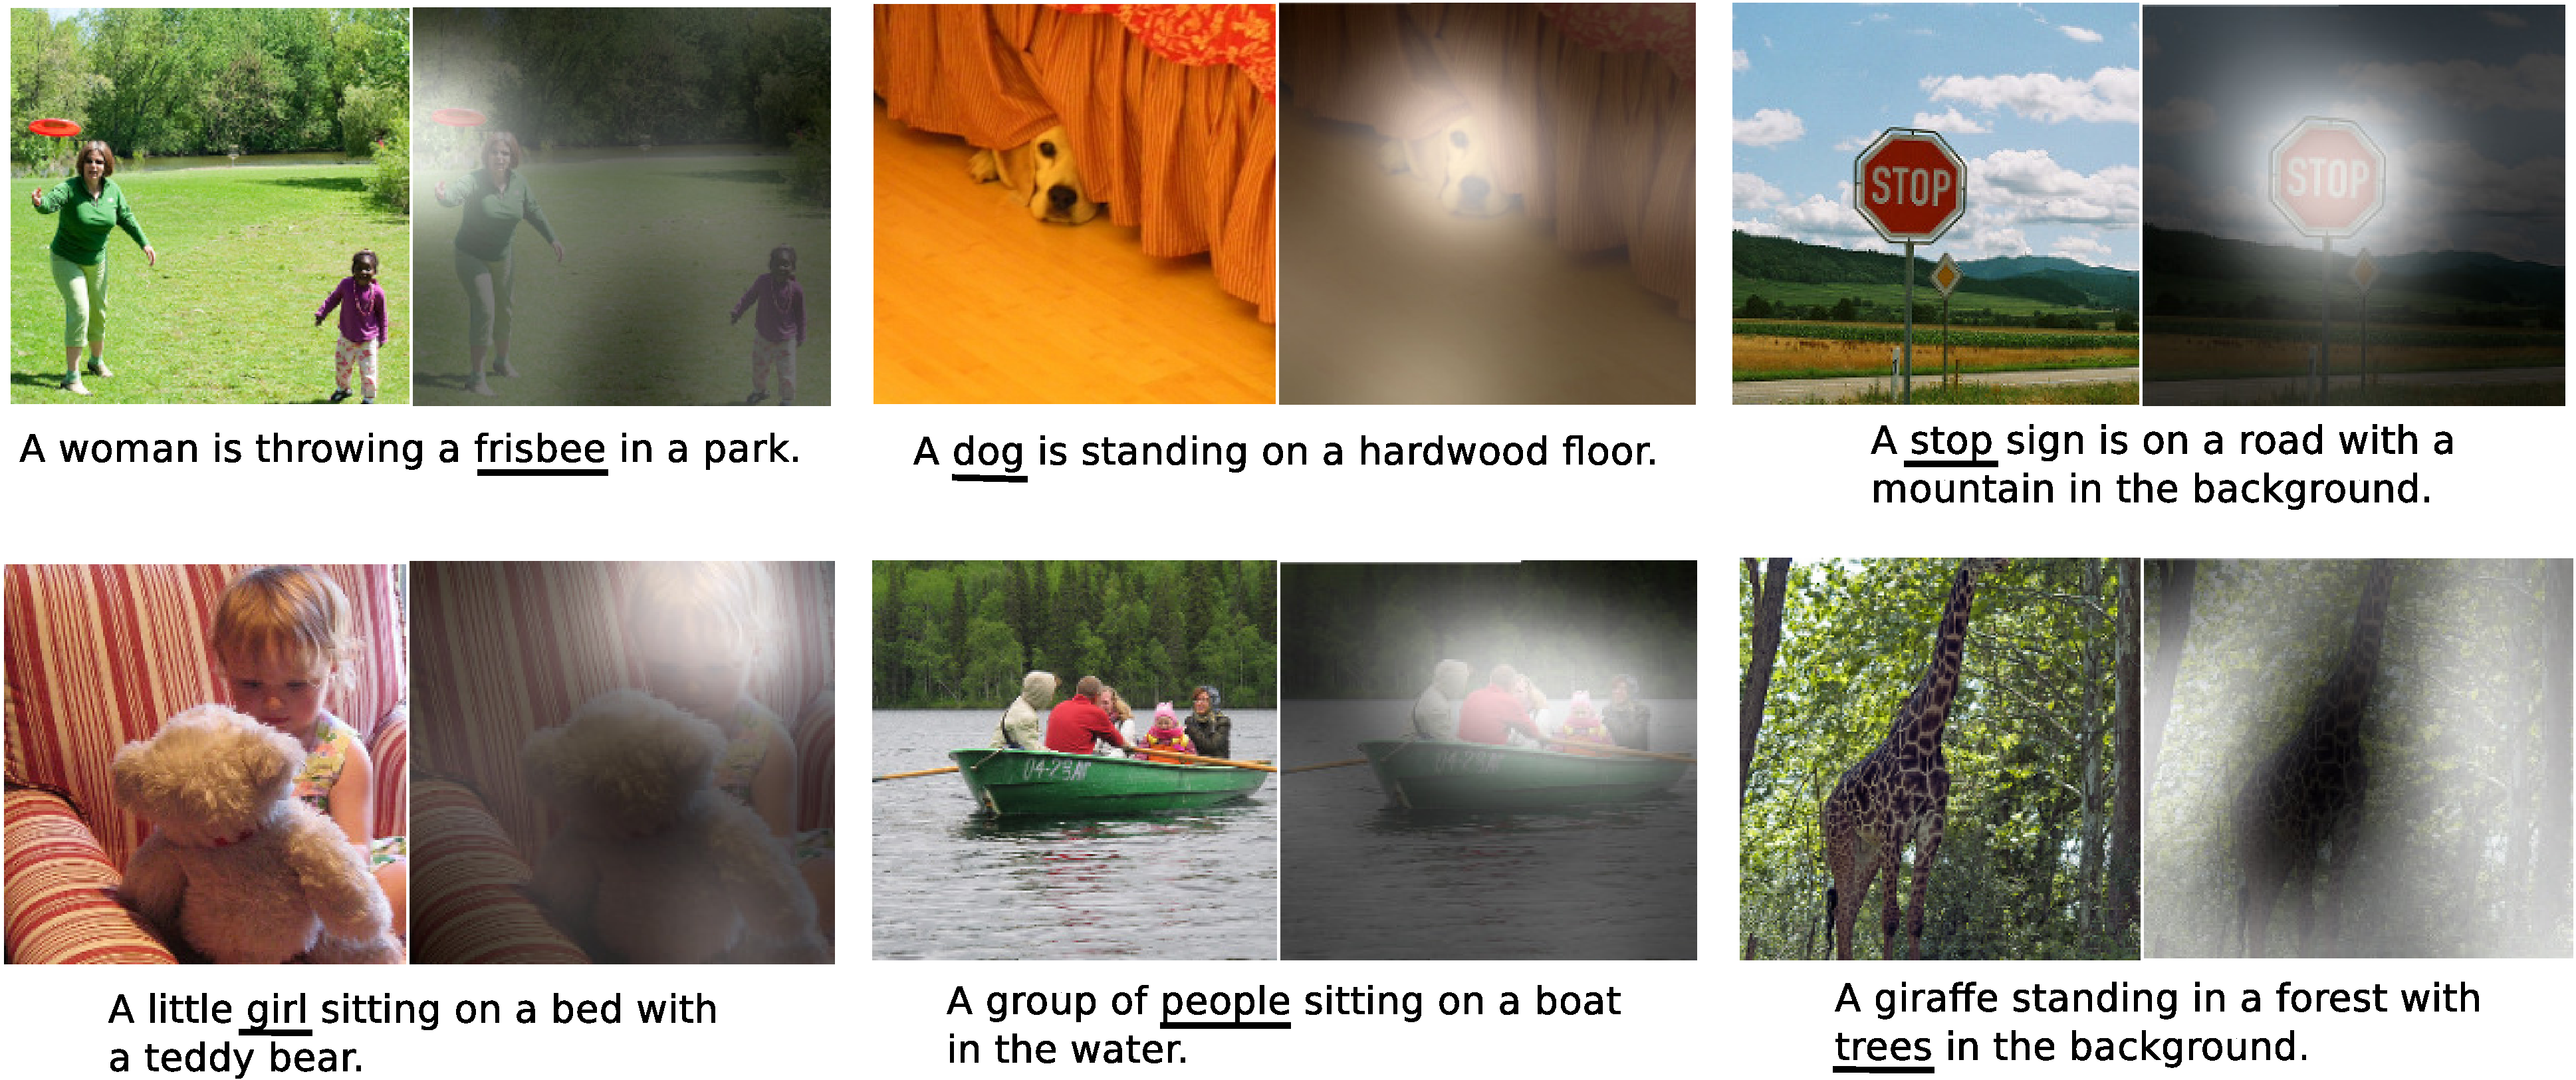
\includegraphics[width=\linewidth]{Images/good_Xu.pdf}
	\caption[Voorbeelden van aandacht op correcte regio.]{Voorbeelden van aandacht op correcte regio. (Wit in de afbeelding is de gefocuste regio, onderlijnde tekst is het overeenkomstige woord)\cite{Xu2015}}
	\label{fig:attention-example}
\end{figure}


\section{Besluit}
%%% Local Variables: 
%%% mode: latex
%%% TeX-master: "masterproef"
%%% End: 
\chapter{Theoretische Achtergrond}
\label{hst-theorie}
Dit hoofdstuk bevat de theoretische concepten die nodig zijn om de gebruikte aanpak zo goed mogelijk te begrijpen. Het bevat een beschrijving van de gebruikte neurale netwerken en van een aantal concepten uit de statistiek.

\section{Neurale Netwerken}
Algemeen gesproken dient een neuraal netwerk als een simulatie van menselijke hersenen. De structuur van een neuraal netwerk probeert de werking van de neuronen en synapsen in het menselijke brein na te bootsen. Neuronen zijn de primitieve eenheden van het menselijke zenuwstelsel. Ze staan in verbinding met elkaar en communiceren met elkaar door middel van elektrische potentiaal. Afhankelijk van de aan- of afwezigheid van potentiaal over de inkomende verbindingen stuurt een neuron al dan niet een signaal door naar het volgende neuron. Deze eenheden zijn zeer makkelijk softwarematig te simuleren.
Elk artificieel neuraal netwerk heeft een trainingsfase nodig waarin het de juiste gewichten leert. Na deze training kan het netwerk ongeziene input omvormen tot de juiste output.


Deze sectie geeft een inleiding tot de gebruikte neurale netwerken. Een eerste deel handelt over het eenvoudigste type neuraal netwerk (feedforward), dat de basis vormt voor een aantal gebruikte varianten. Daarna volgt een toelichting van enkele meer complexe netwerken: recurrente en convolutionele neurale netwerken, alsook Long Short Term Memory netwerken.

\subsection{Feed Forward Neurale Netwerken}
\paragraph{Perceptron} % (fold)
\label{par:perceptron}

Om een feedforward neuraal netwerk te begrijpen is het concept perceptron nodig. Dit is een netwerk bestaande uit een of meer neuronen, met een of meerdere inputs ($x_i$). De output $y$ van een neuron is een gewogen som van alle inputs met gewichten $w_i$, al dan niet gewijzigd met een transferfunctie $f$ (formule \ref{formule:neuron}). Typische voorbeelden van transferfuncties zijn de logistische functie en de hyperbolische tangensfunctie.

\begin{equation}
    y = f(\sum\limits_{i=1}^{n}w_i x_i)
    \label{formule:neuron}
\end{equation}

Het is ook mogelijk om een perceptron met meerdere outputs te gebruiken. Hierbij heeft elke input \'e\'en gewicht per output en kan elke output een verschillende transferfunctie hebben. Figuur \ref{fig:perceptron} toont een perceptron met vijf inputs en drie outputs. Deze architectuur komt exact overeen met drie aparte neuronen die allemaal dezelfde inputs krijgen, maar elk verschillende gewichten en een verschillende transferfunctie $f_i$ gebruiken.

\begin{figure}[ht]
\def\layersep{2.5cm}
\centering
\begin{tikzpicture}[shorten >=1pt,->,draw=black!50, node distance=\layersep]
    \tikzstyle{every pin edge}=[<-,shorten <=1pt]
    \tikzstyle{neuron}=[circle,fill=black!100,minimum size=17pt,inner sep=0pt]
    \tikzstyle{input neuron}=[neuron, fill=lime!65];
    \tikzstyle{output neuron}=[neuron, fill=red!65];
    \tikzstyle{annot} = [text width=4em, text centered]

    %input neurons
    \foreach \name / \y in {1,...,5}
        \path[yshift=0.5cm]
            node[input neuron] (I-\name) at (0,-\y cm){};

    %output neurons
    \foreach \name / \y in {1,...,3}
        \node[output neuron] (O-\name) at (\layersep,-\y-0.5) {$f_{\name}$};

    %links
    \foreach \source in {1,...,5}
        \foreach \dest in {1,...,3}
            \path (I-\source) edge (O-\dest);

    % Annotate the layers
    \node[annot,above of=I-1, node distance=1cm] (i1) {Input};
    \node[annot,right of=i1] (hl2) {Output};
\end{tikzpicture}
\caption{Perceptron met vijf inputs en drie outputs}
\label{fig:perceptron}
\end{figure}


\paragraph{Feedforward Netwerk}
\label{par:concept}
Een feedforward neuraal netwerk is een van de eenvoudigste neurale netwerken. Het is een perceptron met \'e\'en of meer verborgen lagen tussen input en output. De outputs van elke laag worden enkel doorgegeven aan de volgende laag, er zijn dus geen cycli in het netwerk (zie figuur \ref{fig:ffnn}). Elke pijl op de figuur vertegenwoordigt een vermenigvuldiging met een bepaald gewicht. Het is voor elke knoop in het netwerk ook mogelijk om een transferfunctie te gebruiken alvorens de waarde door te sturen naar de volgende laag. Hier is het ook mogelijk om een outputlaag te gebruiken met meerdere knopen, wat neerkomt op een parallelle uitvoering van meerdere netwerken met een enkele output.\cite{Bishop:1995:NNP:525960} Daarnaast hoeft een knoop niet alle outputs van een vorige laag te gebruiken. Wanneer het niet volledig verbonden is, komt dit immers neer op een gewicht van 0 voor de niet-verbonden knopen.

\begin{figure}[ht]
\def\layersep{2.5cm}
\centering
\begin{tikzpicture}[shorten >=1pt,->,draw=black!50, node distance=\layersep]
    \tikzstyle{every pin edge}=[<-,shorten <=1pt]
    \tikzstyle{neuron}=[circle,fill=black!25,minimum size=17pt,inner sep=0pt]
    \tikzstyle{input neuron}=[neuron, fill=lime!65];
    \tikzstyle{output neuron}=[neuron, fill=red!65];
    \tikzstyle{verborgen neuron}=[neuron, fill=blue!50];
    \tikzstyle{annot} = [text width=4em, text centered]

    % Draw the input layer nodes
    \foreach \name / \y in {1,...,4}
    % This is the same as writing \foreach \name / \y in {1/1,2/2,3/3,4/4}
        \node[input neuron] (I-\name) at (0,-\y) {};

    % Draw the hidden layer nodes
    \foreach \name / \y in {1,...,5}
        \path[yshift=0.5cm]
            node[verborgen neuron] (H1-\name) at (\layersep,-\y cm) {};

    % Draw the hidden layer nodes
    \foreach \name / \y in {1,...,5}
        \path[yshift=0.5cm]
            node[verborgen neuron] (H2-\name) at (2*\layersep,-\y cm) {};

    % Draw the output layer node
    \node[output neuron, right of=H2-3] (O) {};

    % Connect every node in the input layer with every node in the
    % hidden layer.
    \foreach \source in {1,...,4}
        \foreach \dest in {1,...,5}
            \path (I-\source) edge (H1-\dest);
    %links van eerste naar tweede hidden layer
    \foreach \source in {1,...,5}
        \foreach \dest in {1,...,5}
            \path (H1-\source) edge (H2-\dest);

    % Connect every node in the hidden layer with the output layer
    \foreach \source in {1,...,5}
        \path (H2-\source) edge (O);

    % Annotate the layers
    \node[annot,above of=H1-1, node distance=1cm] (hl1) {Verborgen laag 1};
    \node[annot,above of=H2-1, node distance=1cm] (hl2) {Verborgen laag 2};
    \node[annot,left of=hl1] {Input laag};
    \node[annot,right of=hl2] {Output laag};
\end{tikzpicture}
\caption{Feedforward Neuraal Netwerk met twee verborgen lagen}
\label{fig:ffnn}
\end{figure}

% paragraph concept (end)

\paragraph{Training} % (fold)
\label{par:training}
Het trainen van een feedforward netwerk gebeurt meestal met terugpropagatie. Deze techniek vergelijkt de verwachte output bij een gekende input met de berekende output. Op basis van dit verschil gebeuren er aanpassingen aan de gewichten in omgekeerde richting: eerst de gewichten van de laatste laag, dan de voorlaatste, \ldots 

Voor een netwerk met \'e\'en verborgen laag geldt het volgende voor de waarden van de verborgen knopen $\mathbf{\hat{h}}$ en voorspelde outputvector $\mathbf{\hat{y}}$ bij inputvector $\mathbf{x}$:
\begin{equation}
    \mathbf{\hat{h}} = f(\mathbf{Wx})
\end{equation}
\begin{equation}
    \boldsymbol{\hat{y}} = f(\boldsymbol{W'\hat{h}}) = f(\boldsymbol{\hat{h}'}) = f(\boldsymbol{W'}f(\boldsymbol{Wx}))
\end{equation}
waarbij $\mathbf{W}$ en $\mathbf{W'}$ de gewichten van de verbindingen tussen respectievelijk de input en de verborgen laag, en de verborgen laag en de output voorstellen. $f$ is telkens de transferfunctie. In deze formule is ze gelijk voor elke laag, maar het is mogelijk om voor elke laag een andere functie te gebruiken.

Het probleem bij het leren van $\mathbf{W}$ en $\mathbf{W'}$ is dat de correcte verborgen vector $\mathbf{h}$ niet gekend is. De training van het netwerk kan dus enkel op basis van de input,de  berekende output en de verwachte output gebeuren.

Een eerste stap is het verkleinen van het verschil $\mathbf{\hat{y}} - \mathbf{y}$ door het aanpassen van \myvector{W'} en \myvector{\hat{h}}. \myvector{W'} wordt gewijzigd met behulp van gradient descent, veronderstellende dat \myvector{\hat{h}} correct is. Gradient descent is een eenvoudig optimalisatie algoritme dat kan dienen om het lokale minimum van een functie te vinden. De minimalisatie gebeurt op een ``gulzige'' manier, door elke stap wijzigingen aan te brengen in de richting van de steilste afdaling. Deze richting komt overeen met de eerste afgeleide van de transferfunctie, berekend in alle variabelen van de output van het netwerk: 

\begin{equation}
df_i = \frac{\partial}{\partial\hat{h_i}'}f(\hat{h_i}')
\end{equation}
In het geval van een logistische transferfunctie $f(x) = \frac{1}{1 + \mathrm e^{-x}}$ geeft dit volgende vector van afgeleiden:
\begin{equation}
  \mathbf{df} = \frac{d}{d\hat{h}'}\mathbf{\hat{y}} = \mathbf{\hat{y}}(1-\mathbf{\hat{y}})
\end{equation}

De formule om de gewichten te updaten ziet er in het algemene geval uit als volgt:
\begin{equation}
  w'_{ji} = w'_{ji} + \sigma(y_j-\hat{y}_j)df_i\hat{h}_i
\end{equation}
Hierbij stelt $\sigma$ de leersnelheid (learning rate) voor. De leersnelheid bepaalt hoe zwaar de aanpassing aan de gewichten doorweegt.
Indien er een logistische transferfunctie wordt gebruikt geeft dit het volgende resultaat:
\begin{equation}
    w'_{ji} = w'_{ji} + \sigma(y_j-\hat{y}_j)\hat{y}_j(1-\hat{y}_j)\hat{h}_i
\end{equation}
Elke stap zorgt deze gradient ervoor dat aanpassing van de gewichten ervoor zorgt dat, bij dezelfde input, de output dichter bij het gewenste resultaat zal liggen.

Vervolgens zorgt gradient descent voor een aanpassing van \myvector{\hat{h}}. Er kunnen echter geen wijzigingen worden aangebracht in \myvector{\hat{h}} zelf, dus wijzigt het algoritme \myvector{W} zodat de fout op \myvector{\hat{h}} het meeste verkleint. Gradient descent leidt tot volgende \myvector{\Delta h}, die de gewenste verandering van \myvector{\hat{h}} weergeeft:
\begin{equation}
    \Delta h_i = \sum\limits_{j}(y_j-\hat{y}_j)\hat{y}_j(1-\hat{y}_j)w'_{ji}
\end{equation}
Op basis van \myvector{\Delta h} en \myvector{\hat{h}} kan \myvector{W} gewijzigd worden met volgende formule:
\begin{equation}
    w_{ji} = w_{ji} + \sigma(\Delta h_j)\hat{h}_j(1-\hat{h}_j)x_i
\end{equation}
Op deze manier verkleint de fout op de output \myvector{\hat{y}-y}, deels door de verandering in \myvector{W} en deels door die in \myvector{W'}. \cite{Blockeel}

Deze techniek wordt toegepast voor elk paar van gekende inputs en outputs zodat kleine wijzigingen op termijn de juiste gewichten leren. Het is ook mogelijk om elke input meerdere keren toe te passen op het netwerk. Deze methode kan bovendien eenvoudig worden uitgebreid naar een netwerk met een arbitrair aantal verborgen lagen. Hierbij propageert de fout van elke laag door naar de gewichten van de vorige laag. Een zelfde techniek maakt het trainen mogelijk van complexere structuren met terugkoppelingen (RNN) of convolutionele lagen (CNN).
% paragraph training (end)

\paragraph{Softmaxlaag}\label{par:softmax}
De softmaxlaag is een laag die vaak als laatste laag in een neuraal netwerk voorkomt. Wanneer het netwerk meerdere outputs heeft, geeft de softmaxlaag een kansverdeling over de verschillende outputs terug in plaats van de oorspronkelijke outputvector. Concreet betekent dit dat de outputwaarden worden genormaliseerd op een manier dat elke waarde positief is en bovendien de som van alle waarden gelijk is aan 1. Dit is bijvoorbeeld nuttig bij het leren van een kansverdeling over een aantal discrete componenten. Ook bij classificatie van input die tegelijkertijd tot meerdere klassen kan behoren is dit van nut.

De softmaxlaag is eigenlijk de softmaxfunctie $s$ in formule \eqref{formula-softmax}. Hierbij is $o$ de outputvector van grootte $n$.
\begin{equation}
s(\textbf{o})_i = \frac{e^{o_i}}{\sum^{n}_{k=1}{e^{o_k}}}
\label{formula-softmax}
\end{equation}

Het gebruik van softmax bij backpropagatie is zeer eenvoudig. De afgeleide van de softmaxfunctie is te zien in formule \eqref{softmax_derivative}. Hierbij is $\delta_{ik}$ de Kroneckerdelta, die gelijk is aan $1$ als $i = k$ en anders gelijk is aan $0$.

\begin{equation}
    \frac{\partial}{\partial o_k}s(\textbf{o})_i =  s(\textbf{o})_i(\delta_{ik} - s(\textbf{o})_k)
    \label{softmax_derivative}
\end{equation}

Bij het gebruik van negatieve logprobabiliteit als foutenfunctie ($L_i$) komt dit neer op volgende zeer eenvoudige afgeleiden van de foutenfunctie:

\begin{equation}
    \frac{\partial L_i}{\partial o_k} = s(\textbf{o})_k - y_i
\end{equation}
met $\textbf{y}$ de correcte output\cite{Bishop:1995:NNP:525960}.

In deze thesis komt een softmax voor als laatste laag bij de gebruikte CNN (sectie \ref{sec:usedcnn}), als laatste laag in het netwerk bij de voorspelling van LDA-topicverdelingen (sectie \ref{sec:LDAprediction}) en als laatste laag in de gebruikte taalnetwerken (sectie \ref{sec:rnn_methodology} en \ref{sec:lstm}).

% CNN
\subsection{Convolutionele Neurale Netwerken}
\label{sec:CNN}
Convolutionele Neurale Netwerken (ConvNets of CNN's) zijn een biologisch ge\" inspireerde trainbare architecturen die invariante afbeeldingskarakteristieken kunnen leren.\cite{LeCun2010} Ze bieden een hi\"erarchische representatie van een afbeelding en zijn van nut in tal van visuele taken.\cite{Ciresan2012,Girshick2014,Zhou2015}

Een CNN is een \emph{deep learning} architectuur bestaande uit verschillende niveaus. De input en output van elk niveau is een verzameling van arrays die men een \emph{feature map} noemt. Op elke output is de feature map een representatie van een bepaald kenmerk van de afbeelding. Elk niveau bestaat standaard uit drie lagen: een filter bank laag, een non-linearity laag en een feature pooling laag. Na een aantal van deze niveaus is er nog een classificatielaag.

Eerst is er een filter bank laag, die een aantal features kan detecteren in de input. In deze filterlaag gebeurt de eigenlijke convolutie. Het netwerk berekent de convolutie van de verschillende features met een aantal kernelfuncties. Elke filterlaag detecteert andere features op alle mogelijke locaties van de input. Figuur \ref{fig:cnnfilters} toont een voorbeeld van een dergelijke kernelfuncties na afloop van het trainingsproces. De bovenste drie rijen filters focussen minder op kleur, terwijl de onderste drie rijen dat wel doen.

\begin{figure}[tb]
    \centering
    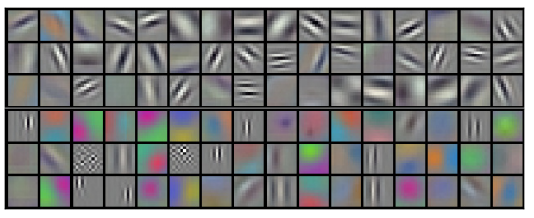
\includegraphics[width=.7\textwidth]{Images/cnnfilters.png}
    \caption{96 convolutionele filters\cite{Krizhevsky2012a}}
    \label{fig:cnnfilters}
\end{figure}

Daarna volgt een niet-lineaire laag. Deze kan een eenvoudige functie bevatten zoals een sigmo\"ide of de $\tanh$ functie, maar kan ook veel complexer zijn en bijvoorbeeld een ``rectified sigmoid'' bevatten, al dan niet gecombineerd met een normalisatie.

De laatste laag in elk niveau is een feature pooling laag die de dimensionaliteit van de output reduceert door regio's van de output te vervangen door hun gemiddelde of maximumwaarde. De maxima (of gemiddelde waarden) van alle regio's vormen dan een down-sampled weergave van de input. Figuur \ref{fig:maxpool} illustreert het principe van max-pooling met een filtergrootte van 2x2 en een stapgrootte van 2. 

\begin{figure}[tb]
    \centering
    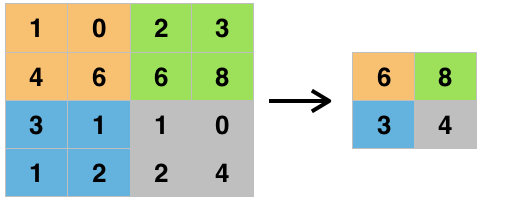
\includegraphics[width=0.6\linewidth]{Images/maxpool.png}
    \caption{Max pooling met 2x2 filter en stapgrootte 2}
    \label{fig:maxpool}
\end{figure}

De laatste fase in een traditionele convolutionele architectuur bestaat uit een aantal volledig verbonden lagen, gevolgd door een classificatielaag.

Trainen van dit netwerk kan gesuperviseerd met behulp van terugpropagatie, maar ook zeer snel ongesuperviseerd waardoor er geen nood is aan zeer grote gelabelde datasets. CNN's zijn in staat om veel sneller concepten te leren dan gewone feedforward netwerken, terwijl ze theoretisch slechts iets mindere resultaten kunnen bekomen. Een CNN gebruikt op elk niveau rechthoekige regio's uit de vorige laag die bovendien mogen overlappen. Door deze overlapping is het netwerk translatie-invariant.

E\'en van de meest succesvolle toepassingen van CNN's is objectdetectie. Deze vooruitgang was vooral te wijten aan een paper\cite{Krizhevsky2012a} die CNN's gebruikt voor het oplossen van de ImageNet challenge.\cite{Russakovsky2014}
Dit is een competitie waarin afbeeldingen moeten worden geclassificeerd in een aantal voorgedefini\"eerde categorie\"en. De gebruikte architectuur bestaat uit 8 lagen waarvan 5 convolutioneel en 3 volledig verbonden. Ze gebruiken bovendien verschillende technieken om overfitten te vermijden. Als classificatielaag gebruiken ze softmax zodat het netwerk een kansverdeling over de verschillende categori\"een leert. De architectuur kan worden gezien in figuur \ref{fig:AlexNet} en  is een variant op de standaardarchitectuur die hierboven werd beschreven. Dit netwerk was het best presterende netwerk voor de wedstrijd in 2012. Ondertussen zijn nog diepere architecturen voorgesteld die op dezelfde en recentere wedstrijden nog betere resultaten bekomen.

Het netwerk (VGGNet)\cite{Arge2015} dat wij gebruiken bestaat uit 16 lagen en is publiek beschikbaar met behulp van Caffe\cite{Jia2014}. De feature maps van verschillende outputlagen van dit netwerk dienen als input voor andere taken dan de ImageNet Challenge. Zo kan de output van de laatste laag voor de classificatielaag worden beschouwd als een representatievector voor de hele afbeelding. Output van de andere lagen is een representatie voor afbeeldingskenmerken op een niveau lager dan de volledige afbeelding.
\begin{figure}[tb]
	\centering
	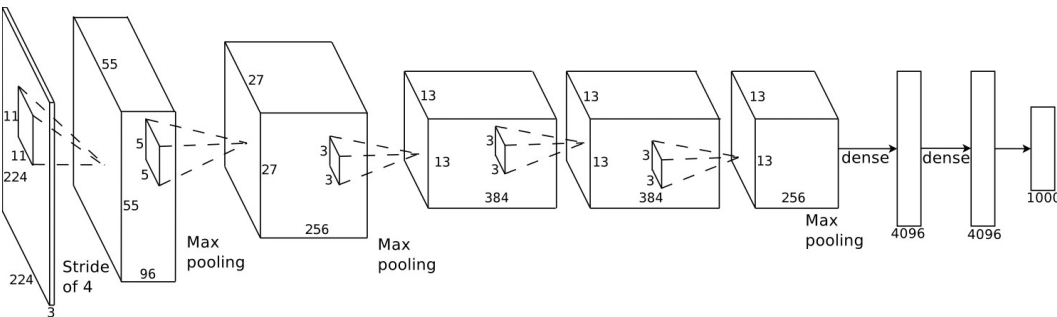
\includegraphics[width=\linewidth]{Images/cnn.PNG}
	\caption{Convolutioneel Neuraal Netwerk gebruikt door \cite{Krizhevsky2012a} voor classificatie van afbeeldingen}
	\label{fig:AlexNet}
\end{figure}

% RNN
\subsection{Recurrente Neurale Netwerken}
\todo[inline]{we hebben buiten word2vec geen enekele referentie in dit stuk?}
\todo[inline]{Referentie zoeken voor RNN}
Recurrente neurale netwerken zijn een uitbreiding van standaard feedforward neurale netwerken. Ze kunnen, net zoals feedforward netwerken, getraind worden met terugpropagatie. Het grote verschil met feedforward netwerken is de terugkoppeling van de output van de vorige stap naar de verborgen lagen. Op figuur \ref{fig:rnn} is een ontrolling van een RNN over verschillende tijdstippen te zien. $U,V$ en $W$ stellen gewichtsmatrices voor. Het ontrollen van het netwerk komt neer op het uitschrijven van het netwerk over verschillende tijdstippen. De pijlen van links naar rechts op de afbeelding komen overeen met de terugkoppeling van de output uit de vorige stap.

De terugkoppeling zorgt ervoor dat het netwerk in staat is om informatie te onthouden. Hierdoor kunnen recurrente netwerken tijdsgerelateerde informatie coderen. Daarom zijn ze geschikt om sequenti\"ele data, zoals tekst, te modelleren en te voorspellen. Recurrente neurale netwerken kunnen bijgevolg gebruikt worden als een taalmodel\cite{Mikolov2010}.

\begin{figure}[tb]
    \centering
    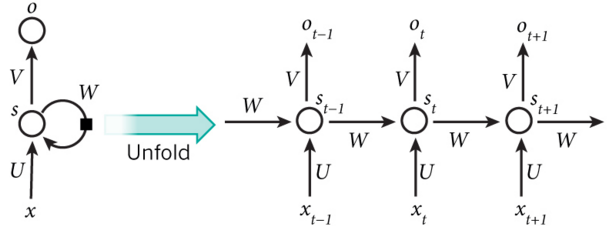
\includegraphics[width=\linewidth]{Images/rnn.PNG}
    \caption{Ontrolling van een recurrent neuraal netwerk\cite{RNNTutorial}}
    \label{fig:rnn}
\end{figure}

Het voorspellen van een zin met een RNN gebeurt woord per woord. Op basis van de eerder waargenomen woorden kan een softmax laag een kansverdeling maken voor het volgende woord. Met behulp van beam-search of het samplen van het meest waarschijnlijke woord, is het netwerk in staat om zinnen te genereren. Tijdens de trainingsfase worden woorden in de vorm van een vector aan het netwerk gegeven. Deze vectoren kunnen gebaseerd zijn op one-hot codering, ze kunnen random zijn, of het kunnen word embeddings zijn zoals bijvoorbeeld \texttt{word2vec}\cite{Mikolov2013}. Deze codering van woorden tot vectoren zelf kan ook deel uitmaken van het netwerk. Als dit het geval is, kan de codering verbeteren tijdens de training met behulp van terugpropagatie.

Een frequent probleem bij het trainen van dergelijke recurrente netwerken is de complexiteit van het netwerk. Hoe complexer het netwerk, hoe groter de kans op ``overfitting''. Hierbij is het uiteindelijke netwerk te hard afgestemd op de trainingsdata, waardoor de precisie op de testdata achteruit gaat. Om dit probleem aan te pakken biedt Srivastava\cite{Srivastava2013} een oplossing. Hij introduceert ``dropout'' om dit fenomeen tegen te gaan. Bij het gebruik van dropout laat het netwerk tijdens het trainen een aantal neuronen vallen. Bij elk trainingsvoorbeeld zijn er een aantal gewichten die waarde 0 krijgen, waardoor ze niet bijdragen aan de training. Een willekeurig proces bepaalt welke neuronen nul zijn in elke stap. Dit proces is aangestuurd door een parameter die de kans op dropout aangeeft per neuron. Deze  kans kan verschillend zijn voor elke laag: typisch is deze kans kleiner voor inputwaarden dan voor verborgen waarden.

Een tweede probleem is het gebrek aan aanpassing van de leersnelheid voor verschillende parameters. Hiervoor zijn een aantal oplossingen te vinden in de literatuur. Eern eerste is het gebruik van ``Adagrad''\cite{Duchi2011}. Hierbij maakt het algoritme gebruik van formule \eqref{formule:adagrad} om de gewichten aan te passen. Hierdoor zullen parameters waarbij de gradi\"ent zeer groot is een lagere effectieve leersnelheid hebben dan parameters met een kleinere gradi\"ent. In de formule staat $w$ voor de gewichtsvector, $dw$ is de grootte van de gradi\"ent, $\sigma$ is de learning rate, en $\epsilon$ is een smoothing parameter die deling door nul voorkomt. Een probleem dat kan voorkomen bij het gebruik van ``adagrad'' is dat het leerproces te vroeg stopt omdat de aanpassingen aan de leersnelheid te agressief zijn.
 
\begin{equation}
    w_t = w_{t-1} - \sigma \frac{dw}{\sqrt{dw^2} + \epsilon}
    \label{formule:adagrad}
\end{equation}

Soms biedt deze methode onvoldoende verbetering, bijvoorbeeld wanneer er negen voorbeelden zijn met gradi\"ent $0.1$ voor een bepaalde parameter, en het tiende voorbeeld heeft waarde $-0.9$. Dan kan ``rmsprop''\cite{RMSprop} een oplossing bieden. Deze techniek maakt gebruik van een bewegend gemiddelde over alle voorbije gradi\"enten om ervoor te zorgen dat grote schommelingen in de gradi\"ent slechts een kleine verandering in de gewichten aanbrengen. Formules \eqref{rmsprop:start}-\eqref{formule:rmsprop} toont hoe dit exact in zijn werk gaat. $\rho$ is de smoothing paramater voor het bewegende gemiddelde, $\sigma$ is de leersnelheid, $a_t$ is het gemiddelde op tijdstip $t$, $dw$ is de gradi\"ent en $w$ is de gewichtsvector. Ook hier vermijdt $\epsilon$ een mogelijke deling door nul.

\begin{eqnarray}
\vspace{-3mm}
    \label{rmsprop:start}
    a_t & = & \rho  a_{t-1} + (1 - \rho)dw^2 \\
    w_t & = &  - \sigma \frac{dw}{\sqrt{a_t} + \epsilon}
    \label{formule:rmsprop}
    \vspace{-3mm}
\end{eqnarray}

Een ander probleem met ``adagrad'' is dat de effectieve leersnelheid naar nul convergeert naarmate de training langer duurt. ``Adadelta''\cite{Zeiler2012} biedt hiervoor een oplossing door, net als rmsprop gebruik te maken van een bewegend gemiddelde, zowel voor gradi\"ent als voor gewichten. Door het gebruik van dit tweede gemiddelde is het niet nodig om expliciet een leersnelheid te defini\"eren. Formules \eqref{adadelta:start}-\eqref{formule:adadelta} tonen de exacte berekening van gewichtsupdates bij het gebruik van adadelta. $a_t$, $\rho$, $\epsilon$, $w$ en $dw$ zijn hetzelfde gedfini\"eerd als bij adagrad. $a_{wt}$ is het bewegende gemiddelde van de gewichten op tijdstip $t$ en $\Delta w_t$ is de aanpassing die gebeurt aan de gewichten op tijdstip $t$.

\begin{eqnarray}
\vspace{-3mm}
    \label{adadelta:start}
    a_t & = & \rho  a_{t-1} + (1 - \rho)dw^2 \\
    \Delta w_t & = & - \frac{\sqrt{a_{w(t-1)} + \epsilon}}{\sqrt{a_{t-1}}}dw \\
    a_{wt} & = & \rho  a_{w(t-1)} + (1 - \rho)\Delta w_t^2 \\
    w_t & = & w_{t-1} + \Delta w_t
    \label{formule:adadelta}
    \vspace{-3mm}
\end{eqnarray}


Twee andere vaak voorkomende problemen bij het trainen van recurrente neurale netwerken zijn exploderende en uitdovende gradi\"enten, waarbij de gradi\"ent van de fout tijdens de training enorm toeneemt, respectievelijk afneemt. Hiervoor zijn een aantal mogelijke oplossingen.

Een mogelijke oplossing is het gebruik van ``gradient clipping'' zoals voorgesteld door Pascanu et al.\cite{Pascanu2012}. Deze methode verkort de gradi\"entvector zodra de lengte van die vector boven een bepaalde drempel $t$ ligt en lost zo het probleem van exploderende gradi\"enten op. De update vindt dan plaats in de dezelfde richting, maar de norm is aangepast. Voor een vector $\mathbf{g}$ komt dit neer op volgende resulterende gradi\"entvector $\mathbf{\hat{g}}$:

\begin{equation}
    \mathbf{\hat{g}} = \frac{t}{||\mathbf{g}||}\mathbf{g}
\end{equation}

Het gebruik van Rectified Linear Units of ReLu-encodering biedt een oplossing voor het probleem van uitdovende gradi\"enten. Dit is een activatiefunctie die werkt volgens formule $ReLu(x) = max(x,0)$. Deze functie is zeer eenvoudig te berekenen en vermijdt uitdovende grade\"enten, in tegenstelling tot niet-lineaire functies zoals een sigmo\"ide of een hyperbolische tangens\cite{Glorot2011}.

Op lange termijn is het voor een RNN moeilijk om informatie te onthouden, net door deze exploderende en verdwijnende gradi\"enten. Hochreiter et al.\cite{SeppHochreiter1997} bieden met Long Short Term Memory netwerken een ander mogelijke oplossing voor dit probleem.

% LSTM
\subsection{Long Short Term Memory Neurale Netwerken}
\label{sub:lstm}
Long Short Term Memory (LSTM) is een vorm van RNN die geheugencellen bevat. Door deze cellen is het netwerk in staat om op lange termijn informatie over de input bij te houden. Elk LSTM blok heeft een aantal gates om te bepalen of de input moet onthouden worden, en of een vorige waarde moet bijgehouden of vergeten worden. De output van de cellen is bijgevolg afhankelijk van alle eerder geobserveerde inputs. Figuur \ref{fig:lstm} toont hoe een LSTM-blok er uitziet.\cite{SeppHochreiter1997,Google}

Op de figuur is duidelijk te zien hoe zowel input als output zijn teruggekoppeld naar de verschillende gates. De waarde van die gates hangt dus af van zowel de vorige voorspelling, als van de nieuwe input.

Formules \eqref{lstm-memory-start}-\eqref{lstm-memory} geven de exacte berekeningen weer die elke stap gebeuren. In deze formules zijn alle $W_{ij}$ gewichtsmatrices, $\sigma$ en $h$ zijn transferfuncties. $x$ is de input van het netwerk, $m_t$ is de output voor de softmaxlaag op tijdstip $t$ en $i'_t$, $f'_t$ en $o'_t$ zijn de waarden van respectievelijk input-, forget- en outputgate op tijdstip $t$. $c'_t$ is de waarde van de geheugencel op tijdstip $t$ en $p_t$ is de uiteindelijke voorspelling van het netwerk op tijdstip $t$. De $\odot$ operator stelt een puntsgewijze vermenigvuldiging tussen twee vectoren voor.

\todo[inline]{f veranderen in een o op tekening}

\begin{figure}[tb]
    \centering
    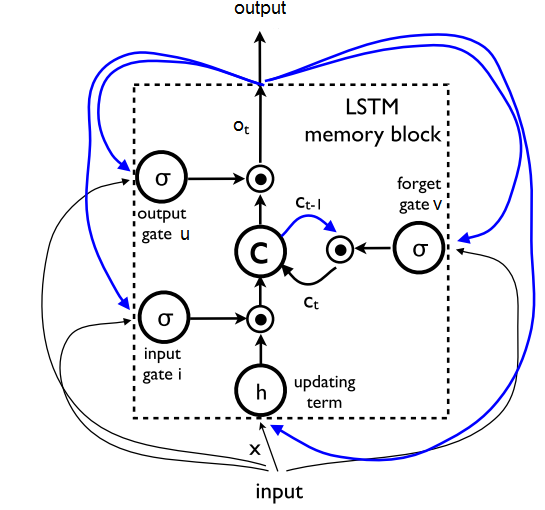
\includegraphics[width=\linewidth]{Images/lstm.PNG}
    \caption{Long Short Term Memory geheugenblok}
    \label{fig:lstm}
\end{figure}

\begin{eqnarray}
\vspace{-3mm}
\label{lstm-memory-start}
i_t' & = & \sigma (W_{ix} x_t + W_{im} m_{t-1}) \label{lstm-input} \\
f_t' & = & \sigma (W_{fx} x_t + W_{fm} m_{t-1}) \\
o_t' & = & \sigma (W_{ox} x_t + W_{om} m_{t-1}) \\
c_t' & = & f_t' \odot c_{t-1}' + i_t' \odot h(W_{cx} x_t + \nonumber \\
&   & + W_{cm} m_{t-1}) \\
m_t & = & o_t' \odot c_t'\\
p_{t+1} & = & SoftMax(m_t)
\label{lstm-memory}
\vspace{-3mm}
\end{eqnarray}

LSTM-netwerken worden net als RNN gebruikt als taalmodellen en zorgen over het algemeen voor hogere kwaliteit. Dit komt doordat LSTM-netwerken over een langere periode dan een gewoon RNN informatie kan onthouden. Dit maakt het modelleren van sequenties met events, die gescheiden zijn door een langere periode, mogelijk.


\section{Statistiek}

% LDA
\subsection{Latent Dirichlet Allocation}
Latent Dirichlet Allocation\cite{Blei2012} is een generatief probabilistisch model voor discrete data. E\'en van de meest gebruikte toepassingen hiervan is het modelleren van een een verdeling van onderwerpen in een set van tekstdocumenten. Dit concept veronderstelt dat elk document een zekere kansverdeling heeft over alle mogelijke onderwerpen. Deze onderwerpen hebben op hun beurt een kansverdeling over alle mogelijke woorden. Zo beschrijft formule \ref{formule:lda} de kans dat een bepaald document $d_j$ een bepaald woord $w_i$ bevat. 

\begin{equation}
    P(w_i | d_j) = \sum\limits_{k=0}^{n_{topics}}P(w_i|topic_k)P(topic_k|d_j)
    \label{formule:lda}
\end{equation}

Het generatieve aspect van LDA is te zien in algoritme \ref{algo:lda} en is ook ge\"illustreerd in figuur \ref{fig:lda}. Op basis van twee Dirichlet priors $\alpha$ en $\beta$ word een kansverdeling over de onderwerpen gesampled per document ($\theta$), alsook een kansverdeling over de woorden voor elk onderwerp ($\phi$). Deze priors geven de onzekerheid over de variabelen ($\theta$ en $\phi$) weer en dienen als basis voor een Dirichletverdeling\cite{Huang}. Een mogelijke interpretatie $\alpha$ is het aantal observaties van de verschillende topics alvorens het document in kwestie is gezien. Hetzelfde met $\beta$, dat het voorafgaand aantal samples van een bepaald woord uit een bepaald topic kan voorstellen. Uit $\theta$ wordt voor elke positie $i$ in een document $j$ een onderwerp gesampled ($z_{ji}$). Het samplen van de woordverdeling voor dit onderwerp leidt tot het woord $w_{ji}$\cite{LDAsien}.

\begin{algorithm}
\caption{Generatief aspect van LDA}
\begin{algorithmic} 
\STATE sample $K$ keer  $\phi \sim Dirichlet(\beta)$
\FORALL{document $d_j$}
\STATE sample $\theta \sim Dirichlet(\alpha)$
\FORALL{woord $i \in d_j$}
\STATE sample $z_ji \sim Multinomial(\theta)$
\STATE sample $w_ji \sim Multinomial(\phi,z_ji)$
\ENDFOR
\ENDFOR
\end{algorithmic}
\label{algo:lda}
\end{algorithm}

\begin{figure}[tb]
    \centering
    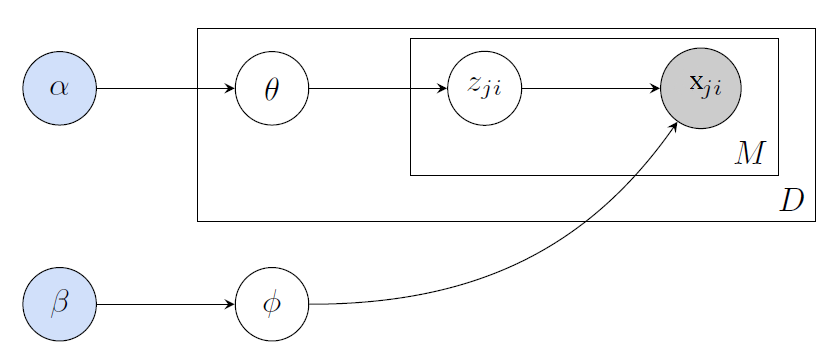
\includegraphics[width=\linewidth]{Images/lda.png}
    \caption{Grafische weergave van LDA}
    \label{fig:lda}
\end{figure}

Trainen van een LDA model gebeurt met een Markov chain Monte Carlo algoritme. Dit type algoritme construeert een Markovketen met als doel een kansdichtheidsfunctie te benaderen. De meest gebruikte techniek om een LDA model te benaderen is Gibbs sampling. Het uiteindelijke doel is het benaderen van de kansverdelingen $\theta$ en $\phi$.

Het trainen met Gibbs sampling begint met een random initialisatie van de topicverdeling voor elk document. Daarna itereert het algoritme over elk woord in elk document. Het berekent de kansverdeling over de verschillende topics, gebaseerd op de onderwerpen van de andere woorden in de collectie (update stap). De exacte berekening is terug te vinden in formule \eqref{lda:update}. Hierbij is $n_{j,k}$ het aantal toekenningen van onderwerp $k$ aan een woord in document $d_j$. $n_{j,k,\neg i}$ is het aantal keer dat topic $k$ is toegekend aan een woord in document $d_j$, woord $w_{ji}$ niet meegeteld. $n_{j,\cdot,\neg i}$ is de som van $n_{j,k,\neg i}$ over alle $K$ topics. $v_{k,w_{ji}}$ is het aantal associaties van woord $w_{ji}$ met topic $k$ in alle documenten, $v_{k,w_{ji}}$ is hetzelfde getal, maar dan zonder het huidige woord $w_ji$ mee te tellen. $v_{k,\cdot,\neg}$ is het totaal aantal woorden die bij topic $k$ horen, zonder $w_{ji}$ mee te tellen.

\begin{equation}
    P(z_{ji} = k | \mathbf{z}_{\neg ji}, \mathbf{w}, \alpha, \beta) \propto \frac{n_{j,k,\neg i} + \alpha}{n_{j, \cdot, \neg i} + K \alpha} \cdot \frac{v_{k,w_{ji}, \neg}+ \beta}{v_{k,\cdot,\neg} + |V|\beta}
    \label{lda:update}
\end{equation}

Op basis van deze kansverdeling wordt een nieuw topic gesampled voor het huidige woord, volgens formule \eqref{lda:sample}. Dit proces van updaten en samplen herhaalt zich tot er convergentie plaatsvindt. De geleerde topicverdelingen voor elk woord dienen dan als basis voor de topicverdelingen voor elk document en de woordverdelingen per topic. De berekening van de document-topicverdeling is te zien in formule \eqref{form:doctopic}, die voor topic-woordverdelingen in formule \eqref{form:topicword}. De symbolen hebben dezelfde betekenis als eerder beschreven.

\begin{equation}
    z_{ji} \sim  P(z_{ji} = k | \mathbf{z}_{\neg ji}, \mathbf{w}, \alpha, \beta)
    \label{lda:sample}
\end{equation}

\begin{equation}
    P(z_k|d_j) = \theta_{j,k} = \frac{n_{j,k} + \alpha}{\sum_{k^*=1}^K n_j,k^* + K\alpha}
    \label{form:doctopic}
\end{equation}

\begin{equation}
    P(w_i|z_k) = \phi_{k,i} = \frac{v_{k,w_i} + \beta}{\sum_{i^*=1}^{|V|} v_k,w_{i^*} + |V|\beta}
    \label{form:topicword}
\end{equation}


Het meest interessante voor deze masterproef zijn de topicverdelingen per document. Deze kunnen gebruikt worden als extra semantische informatie. De systemen kunnen op basis van dergelijke topicverdelingen een verband leren tussen de topics die voorkomen in de beschrijvingen, en de concepten die aanwezig zijn op de afbeelding. 



%  Stacked CCA
\subsection{Canonical Correlation Analysis}
\label{sub:stackedcca}
Canonical Correlation Analysis (CCA) is een methode die basisvectors probeert te vinden voor twee gerelateerde datasets. De bedoeling is om, bij projectie van overeenkomstige elementen uit beide datasets, een maximale lineaire correlatie te bekomen tussen de twee projecties. 
Op basis van singuliere waardenontbinding van de twee datasets is het mogelijk om deze ruimte te benaderen. Door het gebruik van singuliere waarden is het mogelijk om projecties in de tussenliggende ruimte te reduceren tot hun $n$ eerste componenten. Dit komt doordat een singuliere waarden ontbinding de dimensies van de basis gerangschikt zijn van dominant naar minder dominant. Voor een theoretische uitwerking en mogelijke oplossingsmethodes verwijzen we naar Weenink\cite{Weenink2003}.

In het onderzoek naar image captioning kan dit bijvoorbeeld leiden tot een multimodale mapping van afbeeldings- en beschrijvingsrepresentatie.

\paragraph{Stacked CCA}

Stacked Auxiliary Embedding\cite{Gong2014} kan op basis van extra informatie een verbeterde mapping maken. Een voorbeeld hiervan is een dataset van geannoteerde foto's, versterkt met per foto een set van stukjes van de foto met een bijbehorende beschrijving. De representaties van de foto's en annotaties uit de dataset kunnen verbeterd worden door gebruik te maken van de informatie uit de extra dataset.

Om de uiteindelijke augmentatie te bereiken, zijn er een aantal stappen nodig. Uit de extra dataset volgt een eerste set van CCA projecties ($A$, $B$). Daarna volgt een projectie van de originele dataset ($X$, $Y$) naar de multimodale ruimte, door vermenigvuldiging met $A$ en $B$, resulterend in projecties $AX$ en $BY$. Vervolgens transformeren we $AX$ en $BY$ volgens de niet-lineaire functie $\phi(x)$, zoals voorgesteld in de originele paper.

Concatenatie van de originele dataset met het resultaat van de niet-lineaire transformatie leidt tot $\hat{X} = [X, \phi(XA)], \hat{Y} = [Y, \phi(YB)]$. Een laatste stap in het proces is het berekenen van een CCA projectie die gebaseerd is op $\hat{X}$ en $\hat{Y}$, wat resulteert in $U$ en $V$.

Om de dimensionaliteit van de projectie te verhogen wordt voor $\phi(x)$ een random Fourier Feature (RFF) mapping gebruikt. Deze RFF is een functie gebaseerd op de gemiddelde afstand tot de vijftigste dichtste buur van de inputvector. Voor elke foto en caption wordt gekeken welke andere foto of caption de vijftigste dichtste buur is, om vervolgens het gemiddelde te nemen van alle afstanden. De exacte berekening is $\phi(\mathbf{x})=\sqrt{2}cos(\mathbf{x}R+\mathbf{b})$. Hierin is $R$ een matrix die verkregen wordt door sampling van een normaalverdeling met gemiddelde 0, en standaardafwijking $\sigma^2$, waarbij $\sigma$ overeen komt met de eerder berekende gemiddelde afstand. Vector $b$ is resultaat van sampling uit een uniforme verdeling [0,1].

De projectie van een ongeziene afbeelding is het resultaat van het achtereenvolgens uitvoeren van alle transformaties. Voor vector $\mathbf{x}$ geeft dit $\mathbf{\hat{x}} = U[\mathbf{x}, \phi(A\mathbf{x})]$. Deze representatie kan gebruikt worden als een verbeterde versie van de originele image vector, bijvoorbeeld bij een image retrieval taak.

% ... en zo verder tot
\chapter{Het laatste hoofdstuk}
\label{hoofdstuk:n}
Een hoofdstuk behandelt een samenhangend geheel dat min of meer op zichzelf
staat. Het is dan ook logisch dat het begint met een inleiding, namelijk
het gedeelte van de tekst dat je nu aan het lezen bent.

\section{Eerste onderwerp in dit hoofdstuk}
De inleidende informatie van dit onderwerp.

\subsection{Een item}
De bijbehorende tekst. Denk eraan om de paragrafen lang genoeg te maken en
de zinnen niet te lang.

Een paragraaf omvat een gedachtengang en bevat dus steeds een paar zinnen.
Een paragraaf die maar \'e\'en lijn lang is, is dus uit den boze.

\section{Tweede onderwerp in dit hoofdstuk}
Er zijn in een hoofdstuk verschillende onderwerpen. We zullen nu
veronderstellen dat dit het laatste onderwerp is.

\section{Besluit van dit hoofdstuk}
Als je in dit hoofdstuk tot belangrijke resultaten of besluiten gekomen
bent, dan is het ook logisch om het hoofdstuk af te ronden met een
overzicht ervan. Voor hoofdstukken zoals de inleiding en het
literatuuroverzicht is dit niet strikt nodig.

%%% Local Variables: 
%%% mode: latex
%%% TeX-master: "masterproef"
%%% End: 

\chapter{Besluit}
\label{besluit}
Deze masterproef probeert twee bestaande systemen voor afbeeldingsbeschrijving te verbeteren. Deze systemen gebruiken een convolutioneel neuraal netwerk om een afbeelding om te zetten tot een vectorvoorstelling. Deze voorstelling is de input van een taalmodel op basis van een recurrent neuraal netwerk. Samen met een beam-search-algoritme is dit taalmodel in staat om beschrijvingen te genereren.

De verbeteringen ten opzichte van de bestaande systemen gebeuren op drie manieren. Ten eerste is er het afleiden van extra informatie uit een afbeelding, hetzij door het extraheren van onderwerpen, hetzij door een multimodale projectie. Beide gebruikte methodes zijn variabel in het aantal gebruikte dimensies. Deze masterproef bestudeert dan ook de invloed van de dimensionaliteit van de extra informatie. 
De recente dataset Flickr30kEntities vormt een derde bron van informatie, maar blijkt in deze opstelling te groot om mee te werken.
Een tweede aangebrachte verbetering is het normaliseren van de zinnen tijdens het generatieproces. Dit kan leiden tot zinnen die meer informatie bevatten of tot een betere verdeling van de zinslengtes. Tenslotte bestudeert deze masterproef de mogelijke invloed van een aantal parameters van het generatieproces.

De automatische evaluatiemethodes BLEU en Meteor uit de machinevertaling maken een objectieve vergelijking van de verschillende systemen mogelijk. Daarnaast bieden statistieken over woordgebruik, zinslengte en uniciteit van de gegenereerde zinnen verdere inzichten.

Deze thesis experimenteert ook met de robuustheid van de twee manieren om semantische informatie toe te voegen. Een aantal experimenten bepaalt de invloed van ruis op deze informatie.

Dit hoofdstuk biedt eerst een overzicht van de belangrijkste resultaten en verbeteringen, en hoe die een antwoord geven op de geponeerde onderzoeksvragen. Daarna volgt een overzicht van de mogelijke uitbreidingen.
\section{Resultaten}
Deze sectie biedt een overzicht van de behaalde resultaten. De volgende onderdelen focussen telkens op het beantwoorden van \'e\'en of meerdere onderzoeksvragen, zoals gesteld in sectie~\ref{sec:vragen}.
\subsection{Toevoegen van semantische informatie}
\emph{Welke vormen van semantische informatie kunnen op een haalbare manier verbetering bieden voor bestaande systemen?}

Experimenten met het gebruik van de Flickr30k Entities wijzen uit dat het niet haalbaar is om deze dataset om te zetten naar bruikbare informatie. Het gebruik van zowel afgeleide onderwerpverdelingen en multimodale projecties is computationeel minder complex en biedt mogelijkheden tot integratie.

\emph{Hoe kan semantische informatie worden toegevoegd aan de twee bestudeerde systemen?}

Het toevoegen van een vector met semantische informatie aan het bestudeerde RNN gebeurt door de informatie bij de input op te tellen. Bij het uitbreiden van het LSTM-netwerk volgen we de aanpak van Jia et al.~\cite{Fernando2015}. De vector dient dan als gids voor het netwerk.

\emph{Hoe presteren verschillende types van semantische informatie ten opzichte van elkaar?}

Het gebruik van extra semantische informatie leidt tot verbeteringen in de kwaliteit van de gegenereerde zinnen. 
Bij RNN zorgt het gebruik van de onderwerpen afgeleid uit de afbeeldingen voor een hogere score ten opzichte van het referentiemodel. 
De veronderstelling dat de onderwerpen de gegenereerde zinnen beter doet aansluiten bij de afbeelding is dus correct.
Bij LSTM geven zowel de afgeleide onderwerpen als de multimodale projectie een hogere score dan het referentiemodel. 
De scores van beide technieken om extra informatie toe te voegen liggen bij LSTM zeer dicht bij elkaar, maar het gebruik van onderwerpen scoort lichtjes beter op de metrieken die het dichtst aanleunen bij menselijke evaluatie.

\subsection{Normalisatie}
\emph{Hoe kunnen we langere, minder algemene zinnen genereren?}

Om de lengte van de gegenereerde zinnen beter te doen aansluiten bij die van de trainingsverzameling implementeert deze masterproef een Gaussfunctie. Hierdoor krijgen zinnen die te veel afwijken van de lengteverdeling uit de trainingsset een lagere score. 
Deze methode heeft een zeer grote invloed op de gegenereerde zinnen. De gemiddelde lengte stijgt bij RNN van 7 naar 10 en bij LSTM van 8 naar 10. Voor de belangrijkste evaluatiemethodes verbetert deze normalisatie ook de kwaliteit.

Een tweede vorm van normalisatie probeert de gegenereerde zinnen informatiever te maken. Alle woorden uit de woordenschat krijgen een score op basis van de frequentie van voorkomen in de trainingsverzameling. Woorden die minder voorkomen zijn specifieker en krijgen een hogere score. Op basis van deze scores krijgen de woorden in de gegenereerde zinnen een aangepast gewicht. Deze normalisatie leidt effectief tot zinnen die een groter aantal veelzeggende woorden bevatten. Dikwijls leidt dit ook tot een zin van hogere kwaliteit, maar in een aantal gevallen voegt het systeem schijnbaar willekeurig een aantal woorden met een hoge score toe die weinig met de afbeelding te maken hebben. De evaluatiemetrieken oordelen ook dat de zinnen met deze normalisatie in zijn geheel slechter presteren, maar voor een mens zijn een groot aantal van de zinnen wel van betere kwaliteit.

\subsection{Invloed van parameters}
\emph{Wat is de invloed van het aanpassen van systeemspecifieke parameters?}

Verschillende parameters van het systeem hebben een invloed op de resultaten. Ten eerste is er de grootte van de beam-search bij het zoeken van de beste beschrijvingen. Naarmate de grootte stijgt zijn de scores beter, tot aan een plafond. Afhankelijk van het gebruikte systeem ligt de optimale grootte tussen 25 en 75. Ook de dimensionaliteit van de vector met extra semantische informatie heeft een invloed. Bij het gebruik van onderwerpverdelingen is de invloed variabel. Bij langere zinnen, bijvoorbeeld door Gauss-normalisatie, is het beter om een groter aantal onderwerpen te kiezen. Voor kortere zinnen verzwakt dit effect. Bij multimodale projectie is dit fenomeen niet zichtbaar. De modellen die gebruik maken van 256 dimensies scoren wel beter dan die met 128 en 512 dimensies. Bij 128 dimensies is de informatie wellicht te beperkt. Bij 512 daarentegen komen veel onbelangrijke elementen in de vector die doorwegen in het uiteindelijke resultaat.

\subsection{Robuustheid van semantische informatie}
\emph{Welke invloed ondervinden de beschouwde types semantische informatie van trainingsdata die ruis bevat?}

Beide methodes om semantische informatie toe te voegen aan de bestudeerde systemen ondervinden nadeel van ruis op de trainingsdata. Deze ruis bestaat erin elk woord met een kans van 10\% te vervangen door een willekeurig ander woord. De absolute en relatieve achteruitgang is kleiner bij het gebruik van een multimodale projectie. Dit komt vermoedelijk omdat het netwerk dan slechter in staat is om het verband te leren tussen de trainingszinnen en de vector met extra informatie.

\subsection{Beste resultaten}
Wij beschouwen LSTM met een zelf ge\"introduceerde gidsvector op basis van onderwerpverdelingen met 120 onderwerpen als het best presterende systeem. Gaussnormalisatie en een beam-search met grootte 50 leiden tot de hoogste scores.  De vergelijking van de systemen is gemaakt op basis van de hogere BLEU-scores en Meteor, aangezien die het meest correleren met menselijke beoordelingen. Ons systeem presteert zeer gelijkaardig in vergelijking met de meest recente literatuur. Het moet voornamelijk onderdoen voor aandachtsgebaseerde systemen. 

Het gebruik van ons RNN met onderwerpverdelingen van lengte 120 en Gaussnormalisatie presteert iets slechter, maar is veel sneller te trainen. Wanneer de trainingstijd beperkt is of bij het gebruik van een hele grote dataset kan RNN alsnog een waardig alternatief vormen.

\section{Toekomstig werk}
Deze sectie geeft een korte samenvatting van een aantal punten waar in de toekomst verbeteringen mogelijk zijn.

Het trainen van een model met een bepaalde keuze van parameters duurt steeds ongeveer een week op de gebruikte hardware. Om die reden zijn veel van de instelbare parameters in de implementatie nooit gewijzigd. Het loont dus zeker de moeite om te onderzoeken of door wijziging hiervan de resultaten verbeteren.

De huidige modellen struikelen nog steeds over een aantal problemen. Zo is de kwaliteit van de afbeeldingsvoorstelling zeker belangrijk. Betere convolutionele netwerken kunnen hiervoor zorgen. Daarnaast heeft het huidige systeem last met het toewijzen van kleur aan het juiste object. Ook aantallen vormen dikwijls een probleem. Oplossingen hiervoor zijn dus nog nodig.

Bij het onderzoek naar het ideale aantal onderwerpen van LDA, was 120 het best scorende model met Gauss-normalisatie. Het kan interessant zijn om te kijken of een nog groter aantal deze resultaten nog verhoogt en waar net de bovengrens op dit aantal ligt.

Idf-normalisatie zorgt voor creatievere en meer unieke zinnen. Helaas genereert het ook vaak compleet foute beschrijvingen. 
Verder onderzoek naar variaties op deze normalisatie lijkt nuttig. Wanneer deze fouten zouden verdwijnen, lijken de zinnen immers menselijker.

Zoals beschreven in het literatuuroverzicht en de resultaten scoren de modellen die gebruik maken van aandachtsmechanismes het hoogste. Het gebruik van aandachtsvectoren is echter te complex voor deze masterproef. Het is zeker interessant om te experimenteren met het toevoegen van aandachtsinformatie aan de systemen voorgesteld in deze masterproef. De literatuur leert ons dat verbetering zeker nog mogelijk is. 

Een ander mogelijk vervolg op deze masterproef gaat dieper in op de robuustheid van de verschillende systemen om semantische informatie toe te voegen aan de generatiesystemen.
De aanpak in de experimenten is vrij rudimentair, dus het zou zeker lonen om te onderzoeken wat de invloed is van verschillende gradaties van aanpassingen in de trainingsset, alsook verschillende types van ruis.

Een laatste mogelijke verderzetting van dit werk focust op de toepassing van de automatische afbeeldingsbeschrijving. 
Zo is verder onderzoek nodig naar de integratie van dit en soortgelijke systemen in browsers en applicaties voor blinden en slechtzienden. Facebook~\cite{facebook} gebruikt ondertussen al automatische afbeeldingsbeschrijving in hun toepassingen voor slechtzienden. Hierbij beschrijft een stem wat er zich op een geselecteerde afbeelding bevindt. Een algemene browser die elke foto automatisch omzet in een beschrijving en deze bijvoorbeeld voorleest, heeft dus zeker zijn praktisch nut.

%%% Local Variables: 
%%% mode: latex
%%% TeX-master: "masterproef"
%%% End: 


% Indien er bijlagen zijn:
\appendixpage*          % indien gewenst
\appendix
\chapter{De eerste bijlage}
\label{app:A}
In de bijlagen vindt men de data
% ... en zo verder tot
\chapter{De laatste bijlage}
\label{app:n}
In de bijlagen vindt men de data terug die nuttig kunnen zijn voor de
lezer, maar die niet essentieel zijn om het betoog in de normale tekst te
kunnen volgen. Voorbeelden hiervan zijn bronbestanden,
configuratie-informatie, langdradige wiskundige afleidingen, enz.

\section{Lorem 20-24}
\lipsum[20-24]

\section{Lorem 25-27}
\lipsum[25-27]

%%% Local Variables: 
%%% mode: latex
%%% TeX-master: "masterproef"
%%% End: 


\backmatter
% Na de bijlagen plaatst men nog de bibliografie.
% Je kan de  standaard "abbrv" bibliografiestijl vervangen door een andere.
\bibliographystyle{abbrv}
\bibliography{referenties}

\end{document}

%%% Local Variables: 
%%% mode: latex
%%% TeX-master: t
%%% End: 
